%%%%%%%%%%%%%%%%%%%%%%%%%%%%%%%%%%%%%%%%
%% HiMCM/MidMCM LaTeX Template -- 2026 %%
%% Problem B: Requirement 1 working draft
%% Revised after reviewing user-supplied 2025 B papers, November 7, 2026.
%%%%%%%%%%%%%%%%%%%%%%%%%%%%%%%%%%%%%%%%
\documentclass[12pt]{article}
\usepackage{geometry}
\geometry{left=1in,right=0.75in,top=1in,bottom=1in}
\newcommand{\Problem}{B}
\newcommand{\Team}{1111111} % Replace with the actual Team Control Number.
\usepackage{newtxtext}
\usepackage{amsmath,amssymb,amsthm}
\usepackage{newtxmath}
\usepackage[pdftex]{graphicx}
\usepackage{xcolor}
\usepackage{fancyhdr}
\usepackage{microtype}
\usepackage{xurl}
\usepackage{needspace}
\usepackage{booktabs,tabularx,array}
\usepackage{tikz}
\usetikzlibrary{arrows.meta}
\usepackage[hidelinks]{hyperref}
\setlength{\headheight}{15pt}
\setlength{\parskip}{3pt}
\setlength{\parindent}{1.2em}
\lhead{Team \Team}
\rhead{}
\cfoot{}
\newtheorem{theorem}{Theorem}
\newtheorem{corollary}[theorem]{Corollary}
\newtheorem{lemma}[theorem]{Lemma}
\newtheorem{definition}{Definition}

\begin{document}
\graphicspath{{.}}
\DeclareGraphicsExtensions{.pdf,.jpg,.png}
\thispagestyle{empty}
\vspace*{-16ex}
\centerline{\begin{tabular}{*3{c}}
\parbox[t]{0.3\linewidth}{\begin{center}\textbf{Problem Chosen}\\ \Large \Problem\end{center}}&
\parbox[t]{0.3\linewidth}{\begin{center}\textbf{2026\\ HiMCM/MidMCM\\ Summary Sheet}\end{center}}&
\parbox[t]{0.3\linewidth}{\begin{center}\textbf{Team Control Number}\\ \Large \textcolor{red}{\Team}\end{center}}\\
\hline
\end{tabular}}

\begin{center}
\vspace{1.5em}
{\Large\bfseries Measuring Useful Cooling in Open Systems}\\[0.8em]
{\bfseries Working summary: Requirement 1 only}
\end{center}
An open freezer case must maintain appropriate product temperatures despite heat exchange with its surroundings. Electricity use alone does not show how well it performs this task.

We distinguish thermal demand, electrical input, and delivered storage service. Infiltration, cabinet heat transfer, internal equipment, restocking, and defrost contribute to demand. Equipment condition modifies performance, while temperature differences across product locations determine whether the intended service is delivered.

We identify four quantities that define cooling service efficiency: energy input, service quantity, local service quality, and service duration. Compliant product mass-hours per kilowatt-hour provide one possible freezer measure. Product-specific temperature requirements remain a separate adequacy check. Comparisons require prescribed loading, matched ambient conditions, and complete operating cycles.

A process diagram links operating context to local conditions, target response, and accumulated service. A correspondence table transfers these quantities to public spaces, where useful service becomes thermal-discomfort reduction over people and waiting time. Device-specific mechanisms and a common baseline guide the later comparison.

\medskip
\noindent\textit{Draft status.} Only Requirement 1 is developed here. Requirements 2--5 and the final whole-paper summary remain to be completed. No empirical performance results are claimed.

\clearpage
\pagestyle{fancy}
\rhead{Page \thepage}
\tableofcontents
\clearpage

\section{Understanding Cooling Efficiency}
\label{sec:understand}

An open freezer case succeeds by preserving its products. Low electricity use may reflect a smaller workload, shorter operation, or inadequate temperatures; high heat removal may reflect unwanted environmental heat gains. Cooling efficiency must therefore relate energy input to the storage service actually delivered.

\subsection{Selecting the quantities to evaluate}

Table~\ref{tab:service} identifies four quantities that enter the useful-service numerator or energy denominator in both settings.

\begin{table}[!ht]
\centering
\caption{Evaluation quantities and their transfer to a bus stop.}
\label{tab:service}
\small
\renewcommand{\arraystretch}{1.18}
\begin{tabularx}{\linewidth}{@{}>{\raggedright\arraybackslash}p{0.19\linewidth}
>{\raggedright\arraybackslash}X >{\raggedright\arraybackslash}X@{}}
\toprule
Quantity & Open freezer case & Bus-stop shelter\\
\midrule
Energy input & Electricity used by the case and its attributable refrigeration plant (kWh). & Electricity used by fans, pumps, and other cooling equipment (kWh).\\
Service quantity & Actual mass of products stored under a specified loading protocol (kg). & Number of people present in each occupied zone.\\
Local service quality & Product temperatures relative to product-specific storage requirements. & Thermal discomfort relative to the same setting without active cooling.\\
Service duration & Duration of product storage during the evaluation period (h). & Duration of passenger exposure while waiting (h).\\
\bottomrule
\end{tabularx}
\end{table}

\noindent\textbf{Energy input} includes auxiliaries and attributable plant electricity without overlapping meter readings. \textbf{Service quantity} accounts for workload, subject to prescribed loading limits.

\textbf{Local service quality} requires product temperatures at representative locations, rather than discharge-air temperature alone \cite{ashrae}. Averages can hide a warm shelf, and uniformity does not guarantee acceptable storage; product-temperature requirements remain essential \cite{etl}.

\textbf{Service duration} distinguishes sustained performance from a favorable snapshot. Include restocking, compressor cycling, and defrost recovery, with comparable initial and final thermal states so that stored cold cannot inflate the result.


\begin{figure}[!ht]
\centering
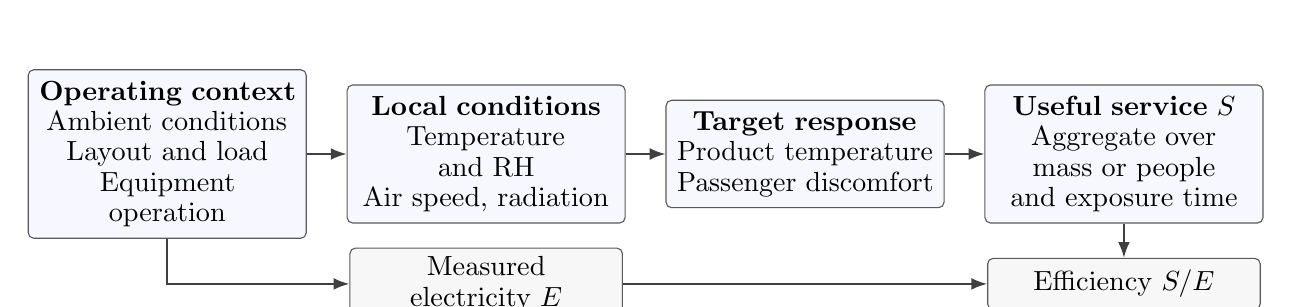
\begin{tikzpicture}[
  font=\fontsize{10}{11}\selectfont,
  stage/.style={draw=black!65,fill=blue!3,rounded corners=2pt,
    text width=3.25cm,minimum height=1.35cm,align=center,inner sep=4pt},
  account/.style={draw=black!65,fill=black!3,rounded corners=2pt,
    text width=3.25cm,minimum height=0.65cm,align=center,inner sep=3pt},
  flow/.style={-{Latex[length=2mm]},line width=0.65pt,draw=black!75}]
\node[stage] (context) at (0,0)
  {\textbf{Operating context}\\Ambient conditions\\Layout and load\\Equipment operation};
\node[stage] (local) at (4.05,0)
  {\textbf{Local conditions}\\Temperature and RH\\Air speed, radiation};
\node[stage] (response) at (8.10,0)
  {\textbf{Target response}\\Product temperature\\Passenger discomfort};
\node[stage] (service) at (12.15,0)
  {\textbf{Useful service} $S$\\Aggregate over\\mass or people\\and exposure time};
\node[account] (energy) at (4.05,-1.65)
  {Measured electricity $E$};
\node[account] (efficiency) at (12.15,-1.65)
  {Efficiency $S/E$};
\draw[flow] (context) -- (local);
\draw[flow] (local) -- (response);
\draw[flow] (response) -- (service);
\draw[flow] (context.south) |- (energy.west);
\draw[flow] (energy.east) -- (efficiency.west);
\draw[flow] (service.south) -- (efficiency.north);
\end{tikzpicture}
\caption{Process linking conditions to service and electricity over the same period ($E>0$).}
\label{fig:process}
\end{figure}

\clearpage
\subsection{Factors that explain performance}

Figure~\ref{fig:process} traces how operating conditions become delivered service. The arrows represent physical dependencies and service accounting; feedback and transient responses are handled within the later models. This process-oriented exposition draws on a supplied AI analysis, with the dependencies revised here \cite{gemini}.

\noindent\textbf{From surroundings to local conditions.} Infiltration carries sensible heat and moisture through the opening; walls transmit heat, and exposed surfaces exchange radiation. Geometry, insulation, ambient temperature, humidity, and airflow therefore alter the conditions around the products and the refrigeration demand \cite{ashrae}.

\noindent\textbf{From operation to local conditions.} Lights and fans release heat, warmer incoming stock adds a temporary load, and defrost interrupts normal cooling \cite{ashrae}. Equipment condition changes insulation, airflow, and power demand. These mechanisms affect both local conditions and measured electricity; age itself is not an additional score.

\noindent\textbf{From local conditions to service.} Product placement and thermal response determine whether the food remains within its required range. Accumulating compliant product mass over time gives useful storage service. The same sequence applies to passengers, but their response depends on the thermal environment and their exposure, rather than food-temperature limits.

\subsection{Implications for the bus-stop model}

The preceding analysis motivates a common evaluation principle:
\begin{equation}
\boxed{\text{Cooling efficiency}
=\frac{\text{useful service accumulated over objects and time}}
{\text{energy input over the same period}}.}
\label{eq:principle}
\end{equation}

The freezer measure can be expressed in compliant kg\,h per kWh. At a bus stop, useful service accumulates thermal-discomfort reduction over people and waiting time. The next model specifies this response and spatial calculation; the two settings do not have numerically comparable units.

First, \textbf{evaluate people directly}. A fan changes local air movement and can improve thermal sensation without lowering air temperature \cite{energystar}. A direct evaporative cooler changes temperature and humidity \cite{evap}. Device-specific mechanisms therefore feed into a common assessment of passenger response.

Second, \textbf{weight effects by occupancy}. Geometry and airflow determine which occupied zones benefit; cooling empty space receives no passenger-service credit. Area is not multiplied by total headcount again. Outdoor air exchange may disperse cooled air while changing local air movement, so its effect is assessed through passenger response.

Third, \textbf{retain a minimum-service check}. Check individual product-temperature excursions and remaining unacceptable passenger exposure even when aggregate service is high. Partial relief can count as a benefit without establishing adequacy; minimum requirements remain separate from the efficiency score.

Within a venue, compare strategies under matched weather, occupancy, geometry, and evaluation periods. Water use, operating cost, and broader visitor experience enter the later effectiveness model. AI-assisted analysis and drafting are recorded in the appended report \cite{codex}.

\clearpage
\phantomsection
\addcontentsline{toc}{section}{References}
\begin{thebibliography}{9}
\bibitem{ashrae}
ASHRAE. \emph{2026 ASHRAE Handbook---Refrigeration},
Chapter 15, \emph{Retail Food Store Refrigeration and Equipment}.
Product Temperatures and Display Refrigerator Cooling Load sections.
\url{https://handbook.ashrae.org/Handbooks/R26/IP/r26_ch15/r26_ch15_ip.aspx}.
Accessed November 7, 2026.

\bibitem{etl}
UK Department for Energy Security and Net Zero.
\emph{Energy Technology List: Retrofit Measures for Open Fronted Refrigerated Display Cabinets}.
Definitions and product-temperature performance requirements.
\url{https://etl.energysecurity.gov.uk/products/refrigeration-equipment/retrofit-measures-open-fronted-refrigerated-display-cabinets}.
Accessed November 7, 2026.

\bibitem{energystar}
ENERGY STAR. \emph{Ceiling Fan Installation and Usage Tips}.
\url{https://www.energystar.gov/products/ceiling_fans/installation-and-usage-tips}.
Accessed November 7, 2026.

\bibitem{evap}
ASHRAE. \emph{2023 ASHRAE Handbook---HVAC Applications},
Chapter 53, \emph{Evaporative Cooling}.
\url{https://handbook.ashrae.org/Handbooks/A23/SI/A23_Ch53/a23_ch53_si.aspx}.
Accessed November 7, 2026.

\bibitem{gemini}
Google Gemini. \emph{AI-generated analysis of the 2026 HiMCM Problem B},
user-supplied PDF conversation excerpt, November 2026.
Consulted for process-oriented exposition; the proposed efficiency formula was
reviewed but not adopted. Exact model identifier was not available in the supplied excerpt.

\bibitem{codex}
OpenAI. \emph{Codex}, AI-assisted formulation, reference checking,
English drafting, and LaTeX preparation, November 2026.
Exact deployed model identifier to be recorded from the session interface.
See the preliminary AI-use record following this draft.

\bibitem{aipolicy}
COMAP. \emph{Use of AI Tools in COMAP Contests}, v102025.
\url{https://www.contest.comap.com/undergraduate/contests/mcm/flyer/Contest_AI_Policy.pdf}.
Accessed November 7, 2026.
\end{thebibliography}

% Add Requirements 2--5, the memorandum, and the blog before References.
% Replace the working summary after completing the full analysis.
\clearpage
\phantomsection
\addcontentsline{toc}{section}{Report on Use of AI Tools}
\section*{Report on Use of AI Tools}
\noindent\textbf{Preliminary record for this partial draft.}

OpenAI Codex assisted with problem translation, the overall modeling discussion,
and the development of Requirement 1 in November 2026. The exact deployed model
identifier must be recorded from the session interface.

For this edit, the user requested an English section in the supplied template
covering infiltration, cabinet heat transfer, internal equipment, restocking,
defrost and operating cycles, equipment age, and spatial temperatures. This is
a summary of the request, not a verbatim transcript.

The assistant proposed and subsequently simplified the evaluation framework,
checked source material, drafted the English text, and prepared the LaTeX.
Separate AI review passes checked technical consistency. At the user's request,
the 2025 Problem B solutions of Teams 16442, 16738, and 16739 were reviewed as
structural references. Their numerical estimates, weighting procedures, and
wording were not used in the present model. This revision emphasizes indicator
justification and transfer to the later task. No field measurements or empirical
performance results were produced.

A user-supplied Google Gemini conversation excerpt was subsequently reviewed.
Its process-oriented explanation informed the organization of the new diagram;
Codex redrew and revised the dependencies and service definitions. The Gemini
model identifier and complete conversation were not available in that excerpt.
The relevant Gemini prompts and outputs must also be included in the final record.

Before submission, add the exact relevant prompts and complete outputs,
including earlier retained contributions and any additional AI tools, as
required by the contest reporting guidance \cite{aipolicy}. Retain this source
file and the chat as records. The student team's independent verification is
still required and has not been asserted in this preliminary record.

\end{document}

